%%%%%%%%%%%%%%%%%%%%%%%%%%%%%%%%%%%%%%%%%%%
%
% From a template maintained at https://github.com/jamesrobertlloyd/cbl-tikz-poster
%
% Code near the top should be fairly standard and not need to be changed
%  - except for the document class
% Code lower down is more likely to be customised
%
%%%%%%%%%%%%%%%%%%%%%%%%%%%%%%%%%%%%%%%%%%%

%%%%%%%%%%%%%%%%%%%%%%%%%%%%%%%%%%%%%%%%%%%
%
% Document class
%
% Change this if you want a different size / orientation poster etc
%
%%%%%%%%%%%%%%%%%%%%%%%%%%%%%%%%%%%%%%%%%%%

\documentclass[landscape,a0b,final,a4resizeable]{a0poster}
%\documentclass[portrait,a0b,final,a4resizeable]{a0poster}

%%%%%%%%%%%%%%%%%%%%%%%%%%%%%%%%%%%%%%%%%%%
%
% 'Basic' packages
%
% TODO - Almost certainly some are unnecessary - feel free to remove nonstandard
% packages if you think it is a good idea not to always have them
%
%%%%%%%%%%%%%%%%%%%%%%%%%%%%%%%%%%%%%%%%%%%
\usepackage{graphicx}
% \usepackage[draft]{graphicx}
\graphicspath{ {fig/} }
 \usepackage[export]{adjustbox}
 
\usepackage{todonotes}
\usepackage[inline]{enumitem}
\usepackage{bm}

\usepackage{sty/msoelch/mlmacros}
\usepackage{amsmath}
\usepackage{mathtools}
\usepackage{calc}
\usepackage{fontawesome}
\usepackage{hyperref}

%\usepackage[osf,sc]{mathpazo} % Palatino as the main font
%\linespread{1.05}\selectfont % Palatino needs some extra spacing, here 5% extra
% \usepackage[euler-digits]{eulervm} % nicer math font

% \usepackage{floatrow}
\usepackage[skip=5pt]{caption}
\usepackage{subcaption}

\usepackage[noabbrev]{cleveref}

% section spacing
\usepackage{titlesec}

\titlespacing*{\section}
{0pt}{.1\baselineskip}{.1\baselineskip}
  
% Decrease spacing between bib entries
%\setlength{\bibsep}{0pt plus 0.3ex}

\newcommand*{\B}[1]{\ifmmode\bm{#1}\else\textbf{#1}\fi}

\variables{a,b,c,g,t,o,s,v,x,z}
\variables{A,I}

\variables[app]{\alpha}
\variables[mean]{\mu}
\variables[std]{\sigma}
\variables[map]{\nu}
\variables[dparam]{\psi}

% Neil's comment function
\newcommand{\nd}[1]{\textcolor{red}{[ND: #1]}}
\newcommand{\ab}[1]{\textcolor{green}{[AB: #1]}}
\newcommand{\ak}[1]{\textcolor{blue}{[AK: #1]}}

\probdists{p,q}

\DeclarePairedDelimiter{\fences}{(}{)}
\DeclarePairedDelimiter{\norm}{\lVert}{\rVert}

%\DeclareMathOperator{\MLP}{ \mathrm{MLP} \Fences }
\newcommand{\MLP}[1]{ \mathrm{MLP} \fences{#1} }
\newcommand{\LSTM}[1]{ \mathrm{LSTM} \fences{#1} }
\newcommand{\flatten}[1]{ \mathrm{vec} \fences{#1} }

\newcommand{\reg}[1]{ \ensuremath{R} \fences{#1} }

\definecolor{darkgreen}{rgb}{0,.502,0}

\newcommand{\sidecaption}[1]% #1 = label name
{\raisebox{\abovecaptionskip}{\begin{subfigure}[t]{1.6em}
  \caption[singlelinecheck=off]{}% do not center
  \label{#1}
\end{subfigure}}\ignorespaces}

\usepackage{multicol}
\usepackage{color}
\usepackage{shadow}
\usepackage{morefloats}
\usepackage{cite}
%\usepackage[pdftex]{graphicx}
\usepackage{rotating}
\usepackage{amsmath, amsthm, amssymb, bm}
\usepackage{array}
\usepackage{nth}
\usepackage[square,numbers]{natbib}
\usepackage{booktabs}


%%%%%%%%%%%%%%%%%%%%%%%%%%%%%%%%%%%%%%%%%%%
%
% TIKZ packages and common definitions
%
% Add extra things as per your tikz needs
%
%%%%%%%%%%%%%%%%%%%%%%%%%%%%%%%%%%%%%%%%%%%

\usepackage{../common/picins}
\usepackage{tikz}
\usetikzlibrary{shapes.geometric,arrows,chains,arrows.meta,matrix,positioning,scopes,calc}
\tikzstyle{mybox} = [draw=none, rectangle]

%%%%%%%%%%%%%%%%%%%%%%%%%%%%%%%%%%%%%%%%%%%
%
% myfig
%
% \myfig - replacement for \figure
% necessary, since in multicol-environment 
% \figure won't work        
%                 
%%%%%%%%%%%%%%%%%%%%%%%%%%%%%%%%%%%%%%%%%%%

\newcommand{\myfig}[3][0]{
\begin{center}
  \vspace{1.5cm}
  \includegraphics[width=#3\hsize,angle=#1]{#2}
  \nobreak\medskip
\end{center}}

%%%%%%%%%%%%%%%%%%%%%%%%%%%%%%%%%%%%%%%%%%%
%
% mycaption                
%
% \mycaption - replacement for \caption
% necessary, since in multicol-environment \figure and
% therefore \caption won't work
%
%%%%%%%%%%%%%%%%%%%%%%%%%%%%%%%%%%%%%%%%%%%

%\newcounter{figure}
\setcounter{figure}{1}
\newcommand{\mycaption}[1]{
  \vspace{0.5cm}
  \begin{quote}
    {{\sc Figure} \arabic{figure}: #1}
  \end{quote}
  \vspace{1cm}
  \stepcounter{figure}
}

%%%%%%%%%%%%%%%%%%%%%%%%%%%%%%%%%%%%%%%%%%%
%
% Some standard colours
%
%%%%%%%%%%%%%%%%%%%%%%%%%%%%%%%%%%%%%%%%%%%

%\definecolor{oriblue}{cmyk}{1., .8, 0., .6}
\definecolor{oriblue}{RGB}{0, 33, 71}
\definecolor{camlightblue}{rgb}{0.601 , 0.8, 1}
\definecolor{camdarkblue}{rgb}{0, 0.203, 0.402}
\definecolor{camred}{rgb}{1, 0.203, 0}
\definecolor{camyellow}{rgb}{1, 0.8, 0}
\definecolor{lightblue}{rgb}{0, 0, 0.80}
\definecolor{white}{rgb}{1, 1, 1}
\definecolor{whiteblue}{rgb}{0.80, 0.80, 1}

%%%%%%%%%%%%%%%%%%%%%%%%%%%%%%%%%%%%%%%%%%%
%
% Some look and feel definitions
%
%%%%%%%%%%%%%%%%%%%%%%%%%%%%%%%%%%%%%%%%%%%

\setlength{\columnsep}{0.03\textwidth}
\setlength{\columnseprule}{0.0018\textwidth}
\setlength{\parindent}{0.0cm}

%%%%%%%%%%%%%%%%%%%%%%%%%%%%%%%%%%%%%%%%%%%
%
% \ - replacement for \section*
% 
% Puts a pretty box around some text
% TODO - any other thoughts for what this box should look like
%
%%%%%%%%%%%%%%%%%%%%%%%%%%%%%%%%%%%%%%%%%%%

\tikzstyle{mysection} = [rectangle, 
									draw=none, 
									shade, 
									outer color=oriblue,
									inner color=oriblue,
									text width=0.965\columnwidth,
									text centered,
									rounded corners=20pt,
									minimum height=0.11\columnwidth]

\newcommand{\mysection}[1]
{
\begin{center}
  \begin{tikzpicture}
    \node[mysection] {\textcolor{white}{\sffamily\bfseries\LARGE#1}};
  \end{tikzpicture}
\end{center}
}

%%%%%%%%%%%%%%%%%%%%%%%%%%%%%%%%%%%%%%%%%%%
%
% Set the font
%
% TODO - Not sure what a canonical choice is - feel free to modify
%
%%%%%%%%%%%%%%%%%%%%%%%%%%%%%%%%%%%%%%%%%%%

\renewcommand{\familydefault}{cmss}
\sffamily

%%%%%%%%%%%%%%%%%%%%%%%%%%%%%%%%%%%%%%%%%%%
%
% Poster environment
%
% Centres everything and can be used to define the width of the content
%
%%%%%%%%%%%%%%%%%%%%%%%%%%%%%%%%%%%%%%%%%%%

\newenvironment{poster}{
  \begin{center}
  \begin{minipage}[c]{0.96\textwidth}
}{
  \end{minipage} 
  \end{center}
}

%%%%%%%%%%%%%%%%%%%%%%%%%%%%%%%%%%%%%%%%%%%
%
% This is probably a good place to put content specific packages and definitions
%
%%%%%%%%%%%%%%%%%%%%%%%%%%%%%%%%%%%%%%%%%%%

\newtheorem{thm}{Theorem}%[section]
\newtheorem{lem}[thm]{Lemma}
\newtheorem{prop}[thm]{Proposition}
\newtheorem{cor}[thm]{Corollary}

\newtheorem*{theorem*}{Theorem}

\theoremstyle{definition}
\newtheorem*{definition*}{Definition}
\newtheorem{definition}[thm]{Definition}%[section]
\newtheorem{conj}{Conjecture}[section]
\newtheorem{exmp}{Example}[section]
\newtheorem{rem}[thm]{Remark}

\theoremstyle{remark}
%\newtheorem{rem}{Remark}
\newtheorem{note}{Note}
\newtheorem{case}{Case}

\newcommand{\eqd}{\overset{\,_{\!d}}{=}}
\newcommand{\defn}[1]{\emph{#1}}

\newcommand{\Law}{\mathcal{L}}

\def\given{\,|\,}

\def\SGinf{\mathbb{S}_{\infty}}

\newcommand{\NonNegInts}{\mathbb{Z}_+}
\newcommand{\Nats}{\mathbb{N}}
\newcommand{\Rationals}{\mathbb{Q}}
\newcommand{\Reals}{\mathbb{R}}

\newcommand{\as}{\textrm{a.s.}}

\def\[#1\]{\begin{align}#1\end{align}}
\newcommand{\defas}{:=}

\newcommand{\Normal}{\mathcal{N}}
\newcommand{\dist}{\ \sim\ }

\newcommand{\kernel}{\kappa}
\newcommand{\kernelmatrix}{K}
\newcommand{\scalefactor}{s}
\newcommand{\lengthscale}{\ell}
\newcommand{\targets}{T}
\newcommand{\noise}{\sigma_\targets}
\newcommand{\pseudopoints}{\eta}
\newcommand{\inputpoints}{\xi}
\newcommand{\covhyppar}{\psi}
\newcommand{\logistic}{\phi}

\newcommand{\CompOrder}{\mathcal{O}}
\def\graphspace{\mathbf{G}}
\def\Uniform{\mbox{\rm Uniform}}
\def\Bernoulli{\mbox{\rm Bernoulli}}
\def\ie{i.e.,\ }
\def\eg{e.g.,\ }
\def\iid{i.i.d.\ }
\def\simiid{\sim_{\mbox{\tiny iid}}}
\def\simind{\sim_{\mbox{\tiny ind}}}
\def\eqdist{\stackrel{\mbox{\tiny d}}{=}}
\def\ahfunction{\theta}       
\def\AHfunction{\Theta}           % A-H random function
\def\AHvar{U}                     % A-H uniform variables
\def\AHvaralt{V}                  % A-H uniform variables - for bipartite data
\def\larray{W}                    % latent array sampled with A-H
%\def\latentspace{\mathbf{W}}      % range of entries
\def\latentspace{\mathcal{W}}      % range of entries
\def\darray{X}                    % data array
%\def\dataspace{\mathbf{X}}        % sample space
\def\dataspace{\mathcal{X}}        % sample space
\def\cfspace{\mathbf{C}}          % space of continuous functions
%\def\GP{\mbox{\mathcal{GP}}}
\def\GP{\mathcal{GP}}
\def\likelihood{P}
\def\CovData{C}
\def\CovDataAlt{D}

\def\newarrow{\mbox{\begin{tikzpicture}
             \useasboundingbox{(-3pt,-4.5pt) rectangle (19pt,1pt)};
             \draw[->] (0,-0.07)--(17pt,-0.07);\end{tikzpicture}}}
         
%%%%%%%%%%%%%%%%%%%%%%%%%%%%%%%%%%%%%%%%%%%
%
% The document environment starts here
%
%%%%%%%%%%%%%%%%%%%%%%%%%%%%%%%%%%%%%%%%%%%

\begin{document}

%%%%%%%%%%%%%%%%%%%%%%%%%%%%%%%%%%%%%%%%%%%
%
% Begin the poster environment - centres things and potentially changes the width
%
%%%%%%%%%%%%%%%%%%%%%%%%%%%%%%%%%%%%%%%%%%%

\begin{poster}

%%%%%%%%%%%%%%%%%%%%%%%%%%%%%%%%%%%%%%%%%%%
%
% Potentially add some space at the top of the poster
%
%%%%%%%%%%%%%%%%%%%%%%%%%%%%%%%%%%%%%%%%%%%

\vspace{0\baselineskip}

%%%%%%%%%%%%%%%%%%%%%%%%%%%%%%%%%%%%%%%%%%%
%
% Draw the header as a TIKZ picture
%
% Using TIKZ to allow for easy alignment
%
%%%%%%%%%%%%%%%%%%%%%%%%%%%%%%%%%%%%%%%%%%%

\begin{center}
\begin{tikzpicture}[x=0.5\textwidth]
    % Dummy nodes at edges for spacing
    % TODO - a better way?
    \node at (+1, 0) {};    
    \node at (-1, 0) {};
    % Set the size of the badges
    \def \badgeheight {0.06\textwidth}
    % Title text
    \node[inner sep=0,text width=0.5\textwidth,text centered,font=\Huge]
%    \node[inner sep=0,
%    text width=0.5\textwidth,
%    text centered,
%    font=\Huge,
%    draw=none,
%    shade,
%    outer color=oriblue,
%    inner color=oriblue] 
    (Title) at (0,0) 
    {
      {\sffamily \Huge \textbf{Hierarchical Attentive Recurrent Tracking}}\\
      {\huge\sffamily Adam R. Kosiorek, Alexy Bewley, Ingmar Posner}\\
      \vspace{-0.3\baselineskip}
      {\large\sffamily Applied AI Lab, Department of Engineering Science, University of Oxford, UK}\\
      \vspace{-0.3\baselineskip}
      {\large \texttt{\{adamk, bewley, ingmar\}@robots.ox.ac.uk}}
      \vspace{-0.5\baselineskip}
    };
    % Cambridge badge
    \node [mybox] (Cambridge Badge) at (-.7, 0) {
        
\includegraphics[height=\badgeheight]{../badges/a2i_logo.pdf}
    };
    % Columbia logo
    \node [mybox] (box) at (0.7, 0) {
        
\includegraphics[width=0.2\textwidth]{../badges/oxford.pdf}
    };
\end{tikzpicture}
\end{center}

%%%%%%%%%%%%%%%%%%%%%%%%%%%%%%%%%%%%%%%%%%%
%
% Spacing between title and main body
%
%%%%%%%%%%%%%%%%%%%%%%%%%%%%%%%%%%%%%%%%%%%

\vspace{1\baselineskip}

%%%%%%%%%%%%%%%%%%%%%%%%%%%%%%%%%%%%%%%%%%%
%
% Columns environment
%
%%%%%%%%%%%%%%%%%%%%%%%%%%%%%%%%%%%%%%%%%%%

\begin{multicols}{3}

%%%%%%%%%%%%%%%%%%%%%%%%%%%%%%%%%%%%%%%%%%%
%
% Start of content
%
%%%%%%%%%%%%%%%%%%%%%%%%%%%%%%%%%%%%%%%%%%%

\Large

%\mysection{Motivation}
\vspace{2\baselineskip}
\section{Introduction}    
    
%    Sequence prediction is a powerful framework for unsupervised learning.
%    Its utility can be intuitively explained by the fact that predicting the future, if it is to be done well, requires a very good understanding of the present. 
%    If a model can learn the idea of an object and infer intuitive physics from data, it should be able to constrain its predictions to the ones where objects obey physically plausible trajectories:\eg a car should not dissolve into thin air.
%    Moreover, the availability and abundance of real-world sequential data make it possible to train large and highly-complex models for this task.
%    While modern approaches based on neural networks have achieved considerable success, they generally do not take any domain-specific problem structure into account, nor do they provide transferable representations that could be easily used for downstream tasks.         
%    
%    Recent advances in variational inference and neural networks allow building scalable generative latent-variable models of high-dimensional data.
%    On one hand, the latent variables explain observations, are typically low-dimensional, and can be used in downstream tasks.
%    On the other, this approach results in an approximation to the true probability distribution of the data, which allows generation of multiple trajectories from a single starting point. 
%    One could argue that stochasticity is not necessary in fully-observable environments. In the real-world, however, partial-observability is most often the case and a stochastic system can act as a simulator conditioned on imperfect information. 
%%    
%    A stochastic and imperfect simulator of this kind can be used for model-based reinforcement learning (RL) as argued by \cite{Sutton1991} to improve sample-efficiency of model-free approaches. 
%    The majority of sequence predictors that act in the image space has the problem, however, that the further in time they venture, the more blurry and undefined the predictions become. 
%    With the increasing divergence between the true data distribution and the predictive distribution the quality of model-free policies decreases and planning becomes inaccurate.
%
%    All work performed under this thesis will aim at constructing a generative latent-variable model of sequential data, where the model structure introduces prior information about the task. Specifically, the structure of the model will encourage learning intuitive physics and decomposing scenes into their constituent components; by modelling moving objects separately, it will be possible to perform counter-factual stochastic simulation. One of the core features of the model is the ability to simulate in the latent space, therefore circumventing the issue of blurry predictions. Since latent variables describe the state of the world, we will aim at conditioning a model-free policy on these latent variables for action prediction. Finally, we will test the generative model of the environment in the Dyna framework \citep{Sutton1991}.
%    
%    The rest of this paper is structured as follows.
%    \Cref{sec:lit} covers prior work related to the areas in question.
%    I summarise the task of sequence prediction, describe relevant variants of unsupervised learning, investigate how model structure helps to learn abstract concepts from data and examine prior work on Dyna.
%    In \cref{sec:done}, I describe our work on object tracking and how it ties with my interests and the planned future work.
%%    \Cref{sec:proposal} details my future research plans, related risks and expected outcomes.
%    \Cref{sec:proposal} details how we are going to build a structured generative model of sequences and use it in model-based RL.
%    \Cref{sec:conclusions} concludes this work.


    Reinforcement learning (RL) allows to learn through the interaction with the environment: an agent controlled by a machine learning (ML) algorithm interacts with the world and develops a policy so as to maximise a reward. 
    Traditional approaches to RL employed hand-designed state-spaces and tabular representations of policies, often based on state-visitation frequencies.
    While useful in theory, this approach is infeasible for complex real-world problems in rich environments. 
    On one hand, designing state-space by hand is difficult as it is not clear what features are important for a particular task or type of the environment. 
    On the other hand, the state-space is either uncountable or too big to enumerate explicitly.
%    
    Model-free deep RL solves these issues by the means of function approximation with neural networks. 
    It can learn representations from sensory inputs directly, thereby eliminating any need for state-space design, but it does it at a cost of a significant decrease in sample efficiency.
    Model-based approaches can potentially improve sample-efficiency of RL algorithms, but they constrain the maximum achievable performance as the resulting policy can be only as good as the model.
    Dyna, a framework combining model-free and model-based approaches introduced by \cite{Sutton1991}, can theoretically achieve optimal performance while using imperfect models of the environments for improved sample-efficiency.
    In practice, it has been hard to use non-linear function approximators within Dyna, however.
    Firstly, the further in future we predict, the lower the quality of the prediction due to increasing uncertainty. 
    While it is true for both linear and non-linear models, the former can provide good uncertainty estimates, which can be used to correct the resulting bias in the predictions. 
    Secondly, non-linear models are sample-inefficient and require significant amount of training before becoming useful. 
    Before that happens, they can destabilise training of the model-free policy by providing inaccurate predictions.

    While it is hard to provide high-quality predictions in the image space, especially over long time-horizons, it is not clear whether it is necessary, or whether all parts of the image have to be predicted with equal accuracy. 
    Consider the task of assembling an object from its parts: 
    there are several parts lying on a workbench and the goal is to arrange them in a specific configuration. 
    While the exact appearance of the final scene or what is in the background does not matter, absolute poses and identities of object parts as well as relations between them do. 
    It is interesting to ask whether we can build a non-parametric latent-variable model of the scene, where latent variables would explain objects and their poses and where the encoding length would depend on the number of objects in the scene (hence non-parametric).
    Moreover, is it possible to perform prediction or a model-based simulation in the latent space, so as to circumvent deteriorating prediction quality, often visible in the image space? 
    Finally, would it be possible to use such latent-space simulations within the Dyna framework, especially with a pre-trained dynamic model of the environment? 
    It is worth noting that decomposing a scene into its constituent parts enforces conditional independence between objects given the scene, making it harder to implicitly reason about relations between objects. 
    It begs asking the following question: does scene decomposition require to consider intra-object relations explicitly or is implicit treatment sufficient?

    To answer the above questions, we would like to focus on the problem of state estimation, and specifically on approaches that 
    (i) can perform multiple number of computation steps per input to support the variable-length representation of the scene, 
    (ii) allow simulation in the absence of data and define prior distributions from which samples can be drawn when data are absent, 
    (iii) support on-line training, which is necessary for a scalable use within the Dyna framework, 
    (iv) estimate a Markovian state, since the environment in many real-world problems, especially involving robots, are partially-observable, 
    (v) are stochastic and thereby able to generate multiple state-space trajectories from a single starting state, which accounts for imperfect information and encourages better state-space exploration necessary for sample-efficient learning of RL models.
    
    While there exist multiple approaches that meet the above requirements, we would like to focus on the recent advances in variational inference for neural networks.
    Variational Autoencoders (VAE) allow building scalable generative latent-variable models of high-dimensional data, which is necessary for our task, and they have been shown to work with variable number of steps per input.  In contrast to standard neural networks, they are stochastic and they provide prior distributions on the latent representation. Unlike Gaussian Processes, they allow on-line training and at the same time the computational complexity of inference is independent of the size of the training set. 

    The rest of this report is structured as follows.
    \Cref{sec:lit} covers prior work related to the areas in question.
    We summarise the task of sequence prediction, describe relevant variants of unsupervised learning, investigate how model structure helps to learn abstract concepts from data and examine prior work on model-based RL.
    In \Cref{sec:done}, We describe our prior work on object tracking and how it ties with our interests and the planned future work.
    \Cref{sec:proposal} details how we are going to build a structured generative dynamics model and use it in reinforcement learning.
    \Cref{sec:conclusions} concludes this work. We provide our prior work on object tracking as an example publication in the Appendix.





\vspace{1\baselineskip}
\mysection{Hierarchical Attention}

\vspace{2\baselineskip}


    \begin{minipage}[c]{0.3\textwidth}
        \centering
        \begin{subfigure}[b]{1.\textwidth}
            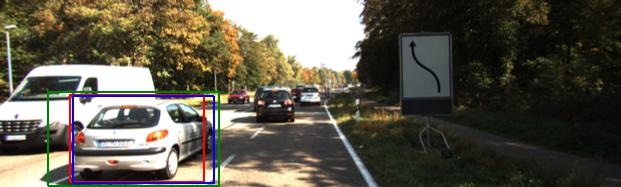
\includegraphics[width=\textwidth]{att_img}
        \end{subfigure}
        
        \hspace{-30pt}
        \begin{minipage}{.85\textwidth}
            \vspace{.5em}
            \begin{subfigure}[b]{.29\textwidth}
                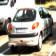
\includegraphics[width=\textwidth, cfbox=darkgreen 4pt 0pt]{att_glimpse}
            \end{subfigure}
            \hfill
            \hspace{8pt}
            \begin{subfigure}[b]{.29\textwidth}
                
\includegraphics[width=\textwidth]{att_mask}
            \end{subfigure}
            \hfill
            \hspace{5pt}
            \begin{subfigure}[b]{.29\textwidth}
                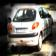
\includegraphics[width=\textwidth]{att_overlay}
            \end{subfigure}
            
        \end{minipage}
    \end{minipage}\hfill
 
    \begin{minipage}[c]{0.3\textwidth}
        \vspace{1em}
            \textcolor{blue}{Ground-truth} and \textcolor{red}{predicted} bounding boxes and an \textcolor{darkgreen}{attention glimpse}. The bottom row shows the three layers of attention: 
            \begin{description}%[labelsep=1em, leftmargin=!,labelwidth=\widthof{\bfseries Interpretable:}]
                \item [$1^{st}$]  layer extracts an attention glimpse (left)
                \item [$2^{nd}$]  layer uses appearance attention to build a location map (middle)
                \item [$3^{rd}$]  layer uses the location map to suppress distractors (right)
            \end{description}
    \end{minipage}


\newpage

\mysection{Two-stream Attentive Model}

\vspace{.5\baselineskip}

\begin{minipage}[c]{0.3\textwidth}
    \centering
    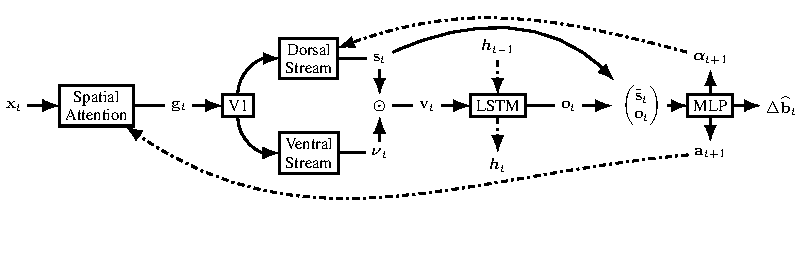
\includegraphics[width=\textwidth]{arch.pdf}
    
    \begin{minipage}[c]{0.5\textwidth}
        \begin{description}
            \item[$\bxt$] input image
            \item[$\bgt$] attention glimpse
            \item[$\bmapt$] appearance-based features
            \item[$\bst$] object segmentation
            \item[$\bvt$] masked features
        \end{description}
    \end{minipage}\hfill
    \begin{minipage}[c]{0.5\textwidth}
                \begin{description}
            \item[$\B{h}_t$] hidden state
            \item[$\bot$] LSTM output
            \item[$\bapp_{t+1}$] appearance
            \item[$\Delta \widehat{\bb}_t$] bounding-box update
            \item[$\ba_{t+1}$] spatial attention
        \end{description}
    \end{minipage}
    
\end{minipage}\hfill

\begin{minipage}{0.3\textwidth}
   \vspace{2em}
   \begin{minipage}[c]{0.5\textwidth}
       \centering
       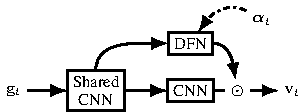
\includegraphics[width=\textwidth]{impl.pdf}
   \end{minipage}\hfill
    \begin{minipage}{0.6\textwidth}
    Appearance attention architecture:
    \vspace{1em}
    \begin{description}[leftmargin=\parindent]
        \item[V1] shared CNN
        \item[Dorsal Stream] Dynamic\\ Filter Network (DFN)
        \item[Ventral Stream] CNN
    \end{description}
    \end{minipage}
\end{minipage}

\vspace{\baselineskip}
%\mysection{Method}

\vspace{0\baselineskip}



\vspace{0\baselineskip}

%\mysection{Is Attention Loss Important?}

\vspace{.5\baselineskip}

\centering
\begin{minipage}[c]{.3\textwidth}
    \centering
    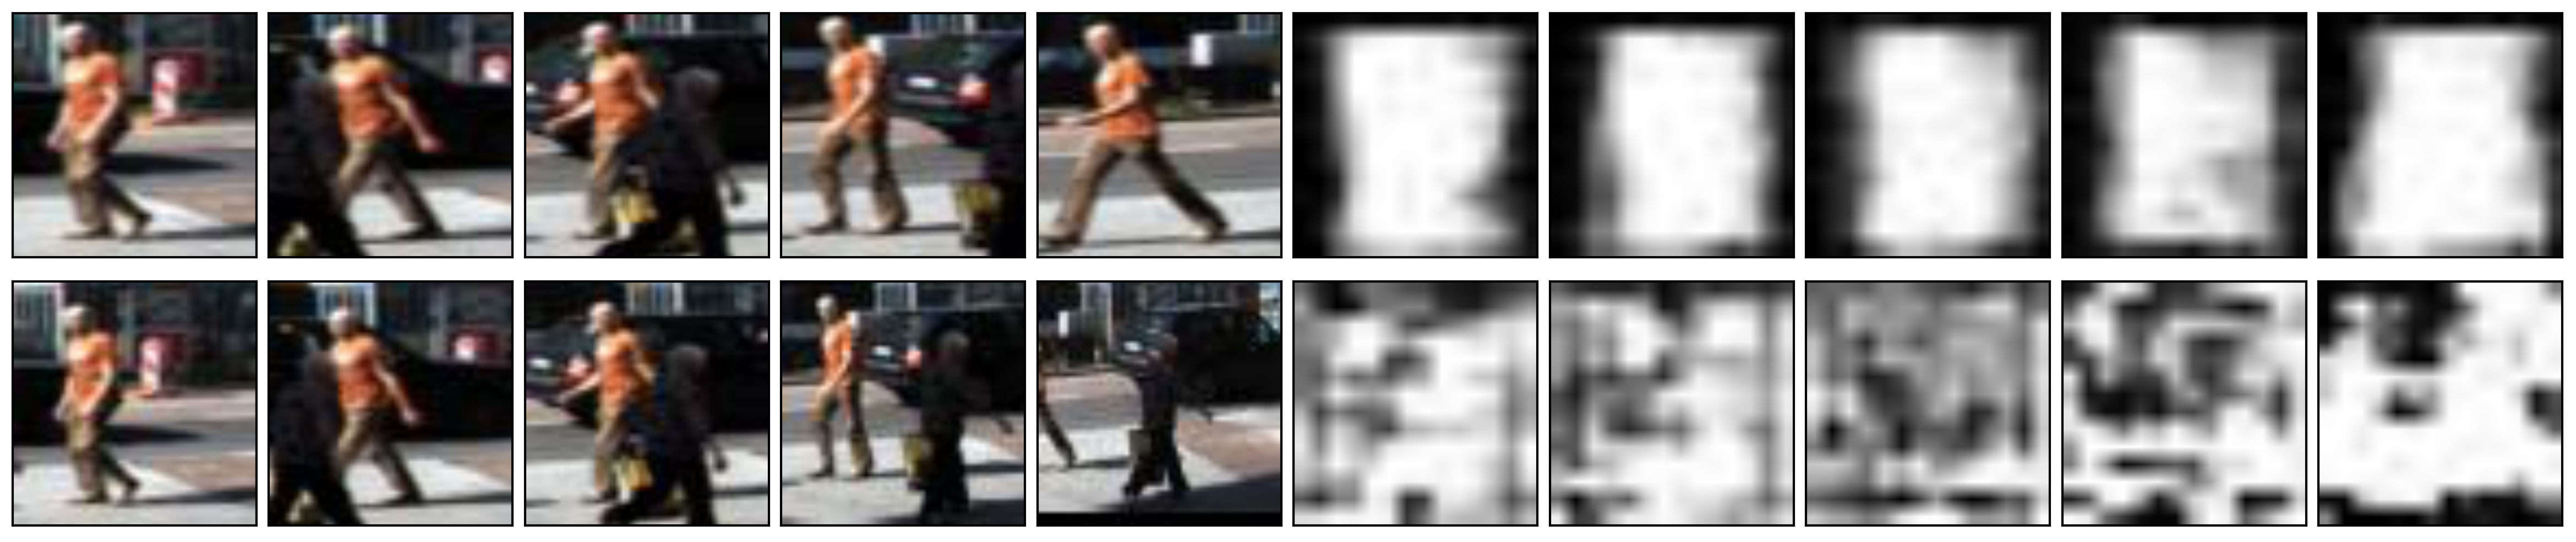
\includegraphics[width=\textwidth]{soft_id_swap}
    \vspace{.5\baselineskip}
    Appearance attention loss (top) prevents an ID swap when a pedestrian is occluded by another one (bottom).
\end{minipage}
\begin{minipage}[c]{.3\textwidth}
    \centering
    \vspace{.5\baselineskip}
    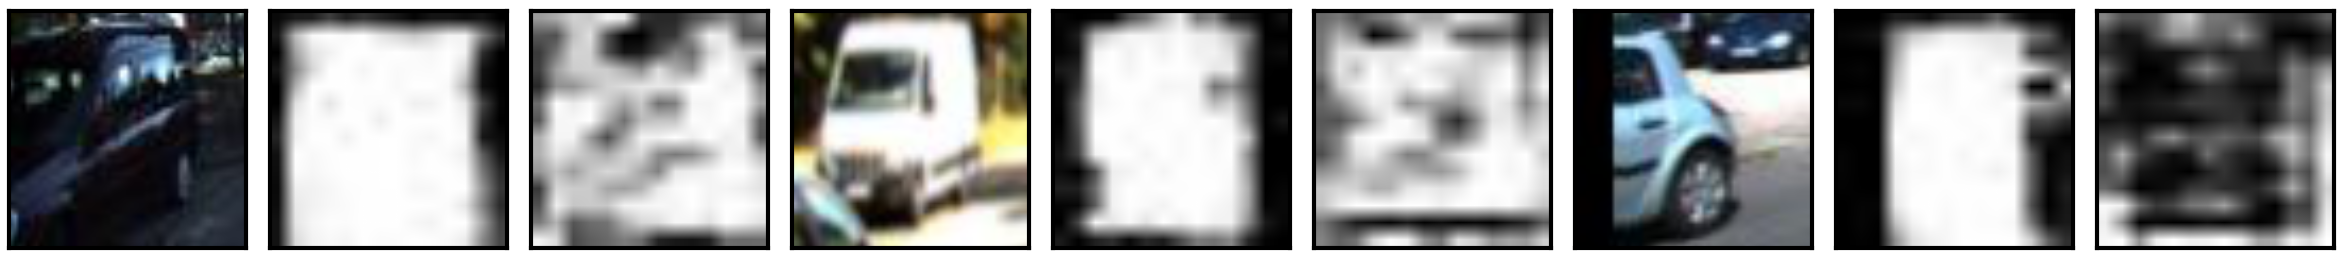
\includegraphics[width=\textwidth]{soft_att}
    \vspace{.5\baselineskip}
   Left to right: glimpses and segmentations learned with and without appearance loss.
   Attention loss leads to distractor suppression. 
\end{minipage}
\mysection{Loss}
\vspace{.5\baselineskip}
    \centering
    Directly optimise Intersection-over-Union (IoU) and guide attention mechanisms.
%\begin{equation*}
%\loss[\mathrm{HART}]{\cdot} = \lambda_{\mathrm{t}} \loss[\mathrm{t}]{\cdot} + \lambda_{\mathrm{s}} \loss[\mathrm{s}]{\cdot} + \lambda_{\mathrm{a}} \loss[\mathrm{a}]{\cdot}  + \reg{ \B{\lambda} } + \beta \reg{ \cdot }
%\end{equation*}
\begin{equation*}
\loss[\mathrm{HART}]{\cdot} = \lambda_{\mathrm{t}} \loss[\mathrm{t}]{\cdot} + \lambda_{\mathrm{s}} \loss[\mathrm{s}]{\cdot} + \lambda_{\mathrm{a}} \loss[\mathrm{a}]{\cdot} + \beta \reg{ \cdot }
\end{equation*}

\begin{description}[leftmargin=\parindent,labelsep=1em]

\item[Tracking:] Negative log of Intersection-over-Union.
\begin{equation*}
    \loss[\mathrm{t}]{\data, \theta} = \expc[\p{\widehat{\bb}_{1:T}}{\bxTs, \bb_1}]{ -\log \mathrm{IoU} \fences{\widehat{\bb}_t, \bbt}}
\end{equation*}

\item[Spatial Attention:] It follows the object, but shouldn't be too big.
\begin{equation*}
    \loss[\mathrm{s}]{\data, \theta} = \expc[\p{\baTs}{\bxTs, \bb_1}]{ -\log \fences*{\frac{ \bat \cap \bbt }{\mathrm{area}\fences{\bbt}} } -\log \fences { 1 - \mathrm{IoU} \fences{\bat, \bxt} } }
\end{equation*}

\item[Appearance Attention:] Cross-entropy with dynamically created target mask $\tau \fences { \bat, \bbt }$:
$\loss[\mathrm{a}]{\data, \theta} =   \expc[\p{\baTs, \bsTs}{\bxTs, \bb_1}]{ H \fences{ \tau \fences { \bat, \bbt }, \bst  } }$.



\begin{minipage}[c]{.3\textwidth}
    \centering
    \vspace{0.75em}
    \caption*{\large With Appearance Attention Loss: Successful Tracking}
    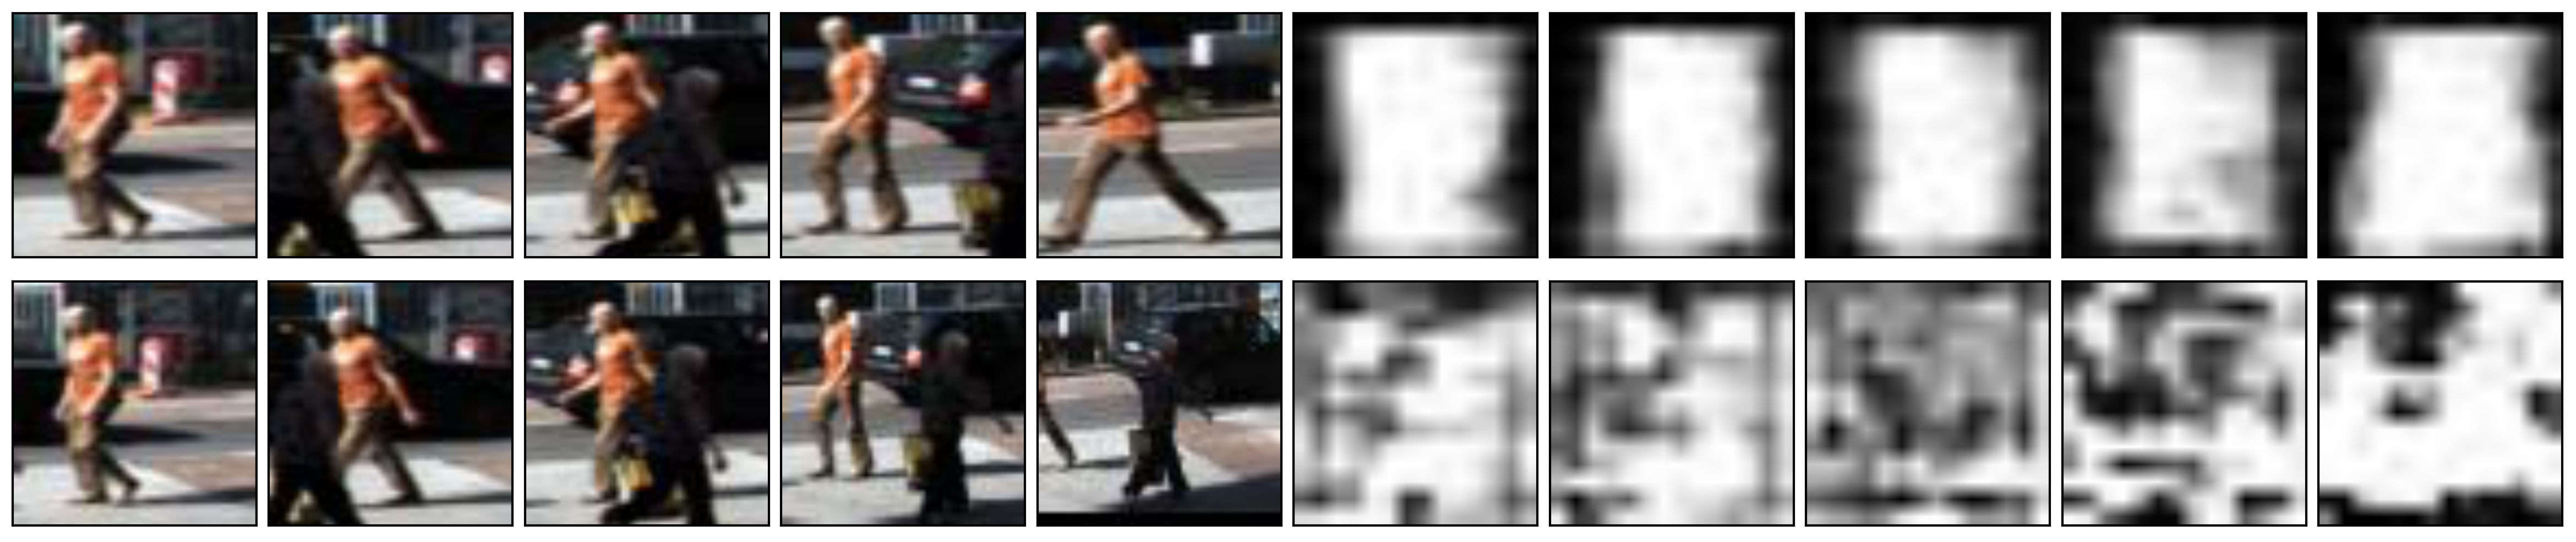
\includegraphics[width=\textwidth]{soft_id_swap}
    \caption*{\large Without Appearance Attention Loss: ID Swap}
\end{minipage}
\end{description}


\vspace{0.5\baselineskip}
{\large \faGithub\ \url{https://github.com/akosiorek/hart} \\ \faYoutube\ \url{https://youtu.be/Vvkjm0FRGSs}}

\newpage

\mysection{Pedestrian Tracking: KTH Dataset [2]}

\vspace{1\baselineskip}

\begin{minipage}[c]{0.3\textwidth}
    \centering
    \vspace{-1.5em}
    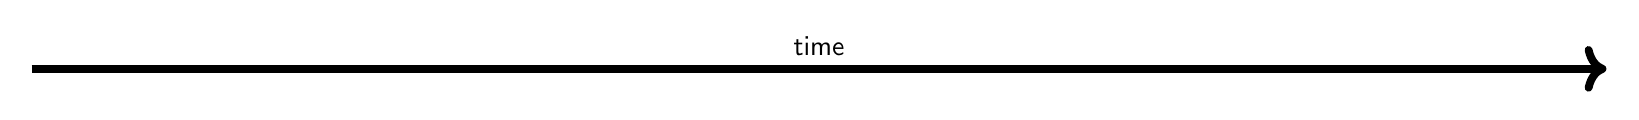
\begin{tikzpicture}
    \draw[line width=1mm, ->] (-10, 0) -- node[above] {time} (10, 0);
    \end{tikzpicture}
    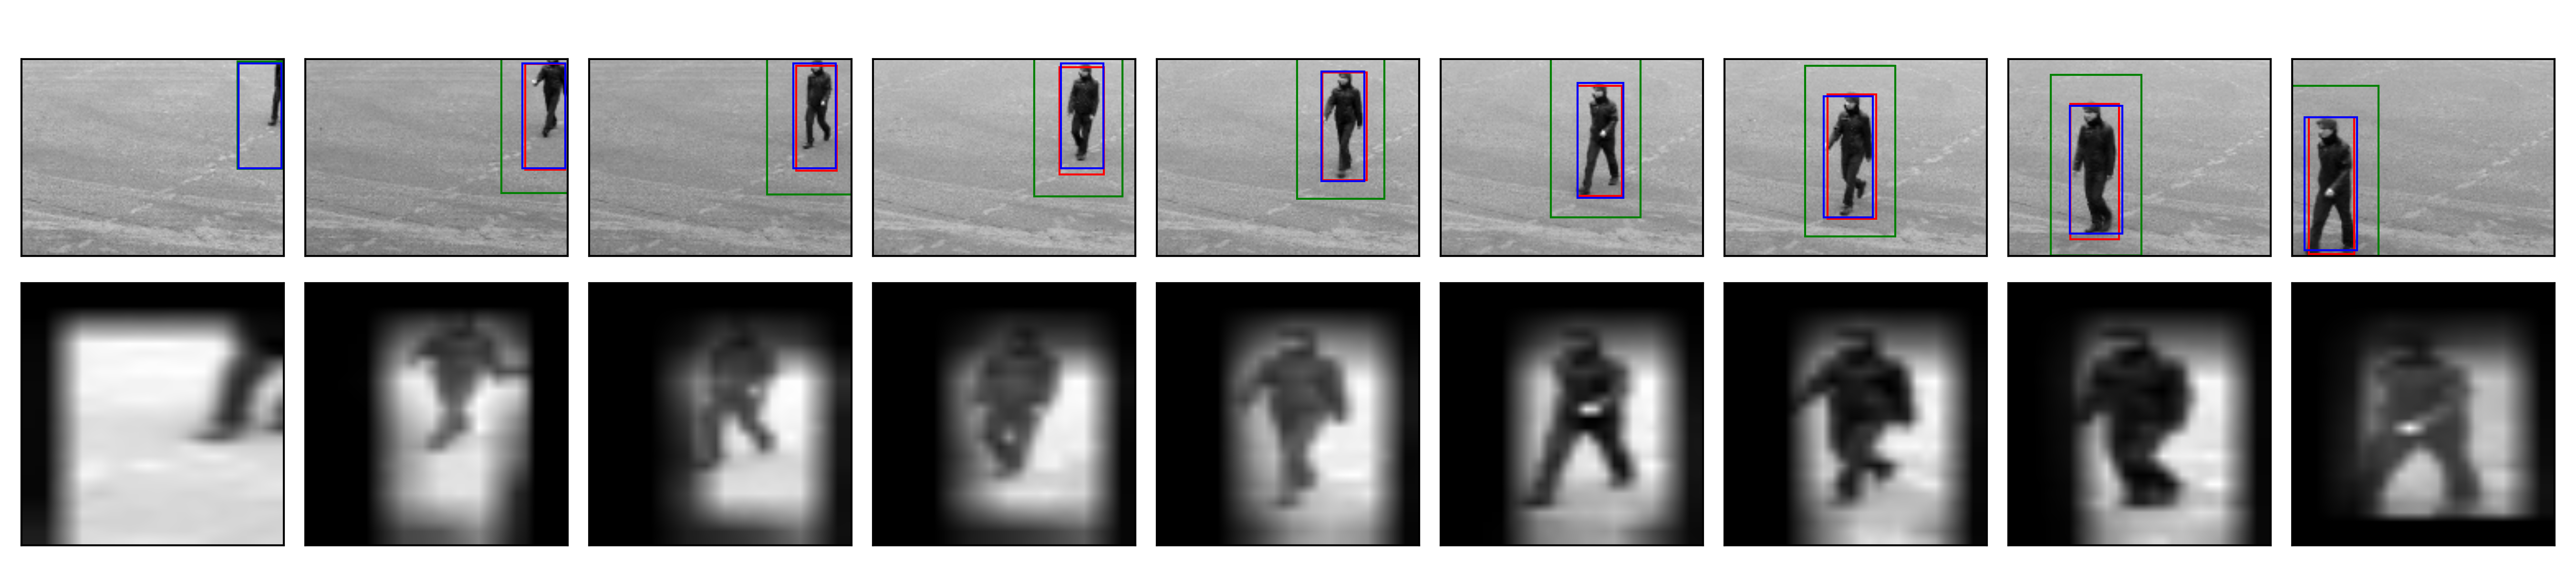
\includegraphics[width=\textwidth]{kth_overlay_16}
    
    \begin{minipage}[c]{0.55\textwidth}
        \begin{itemize}
            \item Attention, prediction and ground-truth overlap at initialization.
            \item Every $16^{th}$ frame of the\\ sequence at 25 fps.
            \item $2^{nd}$ row: attention glimpses multiplied with appearance attention.
        \end{itemize}
    \end{minipage}\hfill   
    {\Large
    \begin{minipage}[c]{0.45\textwidth}
        \begin{tabular}{c|c}
            \multicolumn{2}{c}{Intersection over Union}\\
            Kahou \emph{et. al.} [1] & Ours\\
            \midrule
            0.55 & \B{0.77}
        \end{tabular}
    \end{minipage}
}
    \vspace{.5em}
\end{minipage}



\vspace{0\baselineskip}

\mysection{Scaling to Real-world Data: KITTI [3]}

%\begin{table}
    % \hfill
    \begin{minipage}[c]{0.3\textwidth}
        \centering
        % \todo[inline]{other results are on their way}
        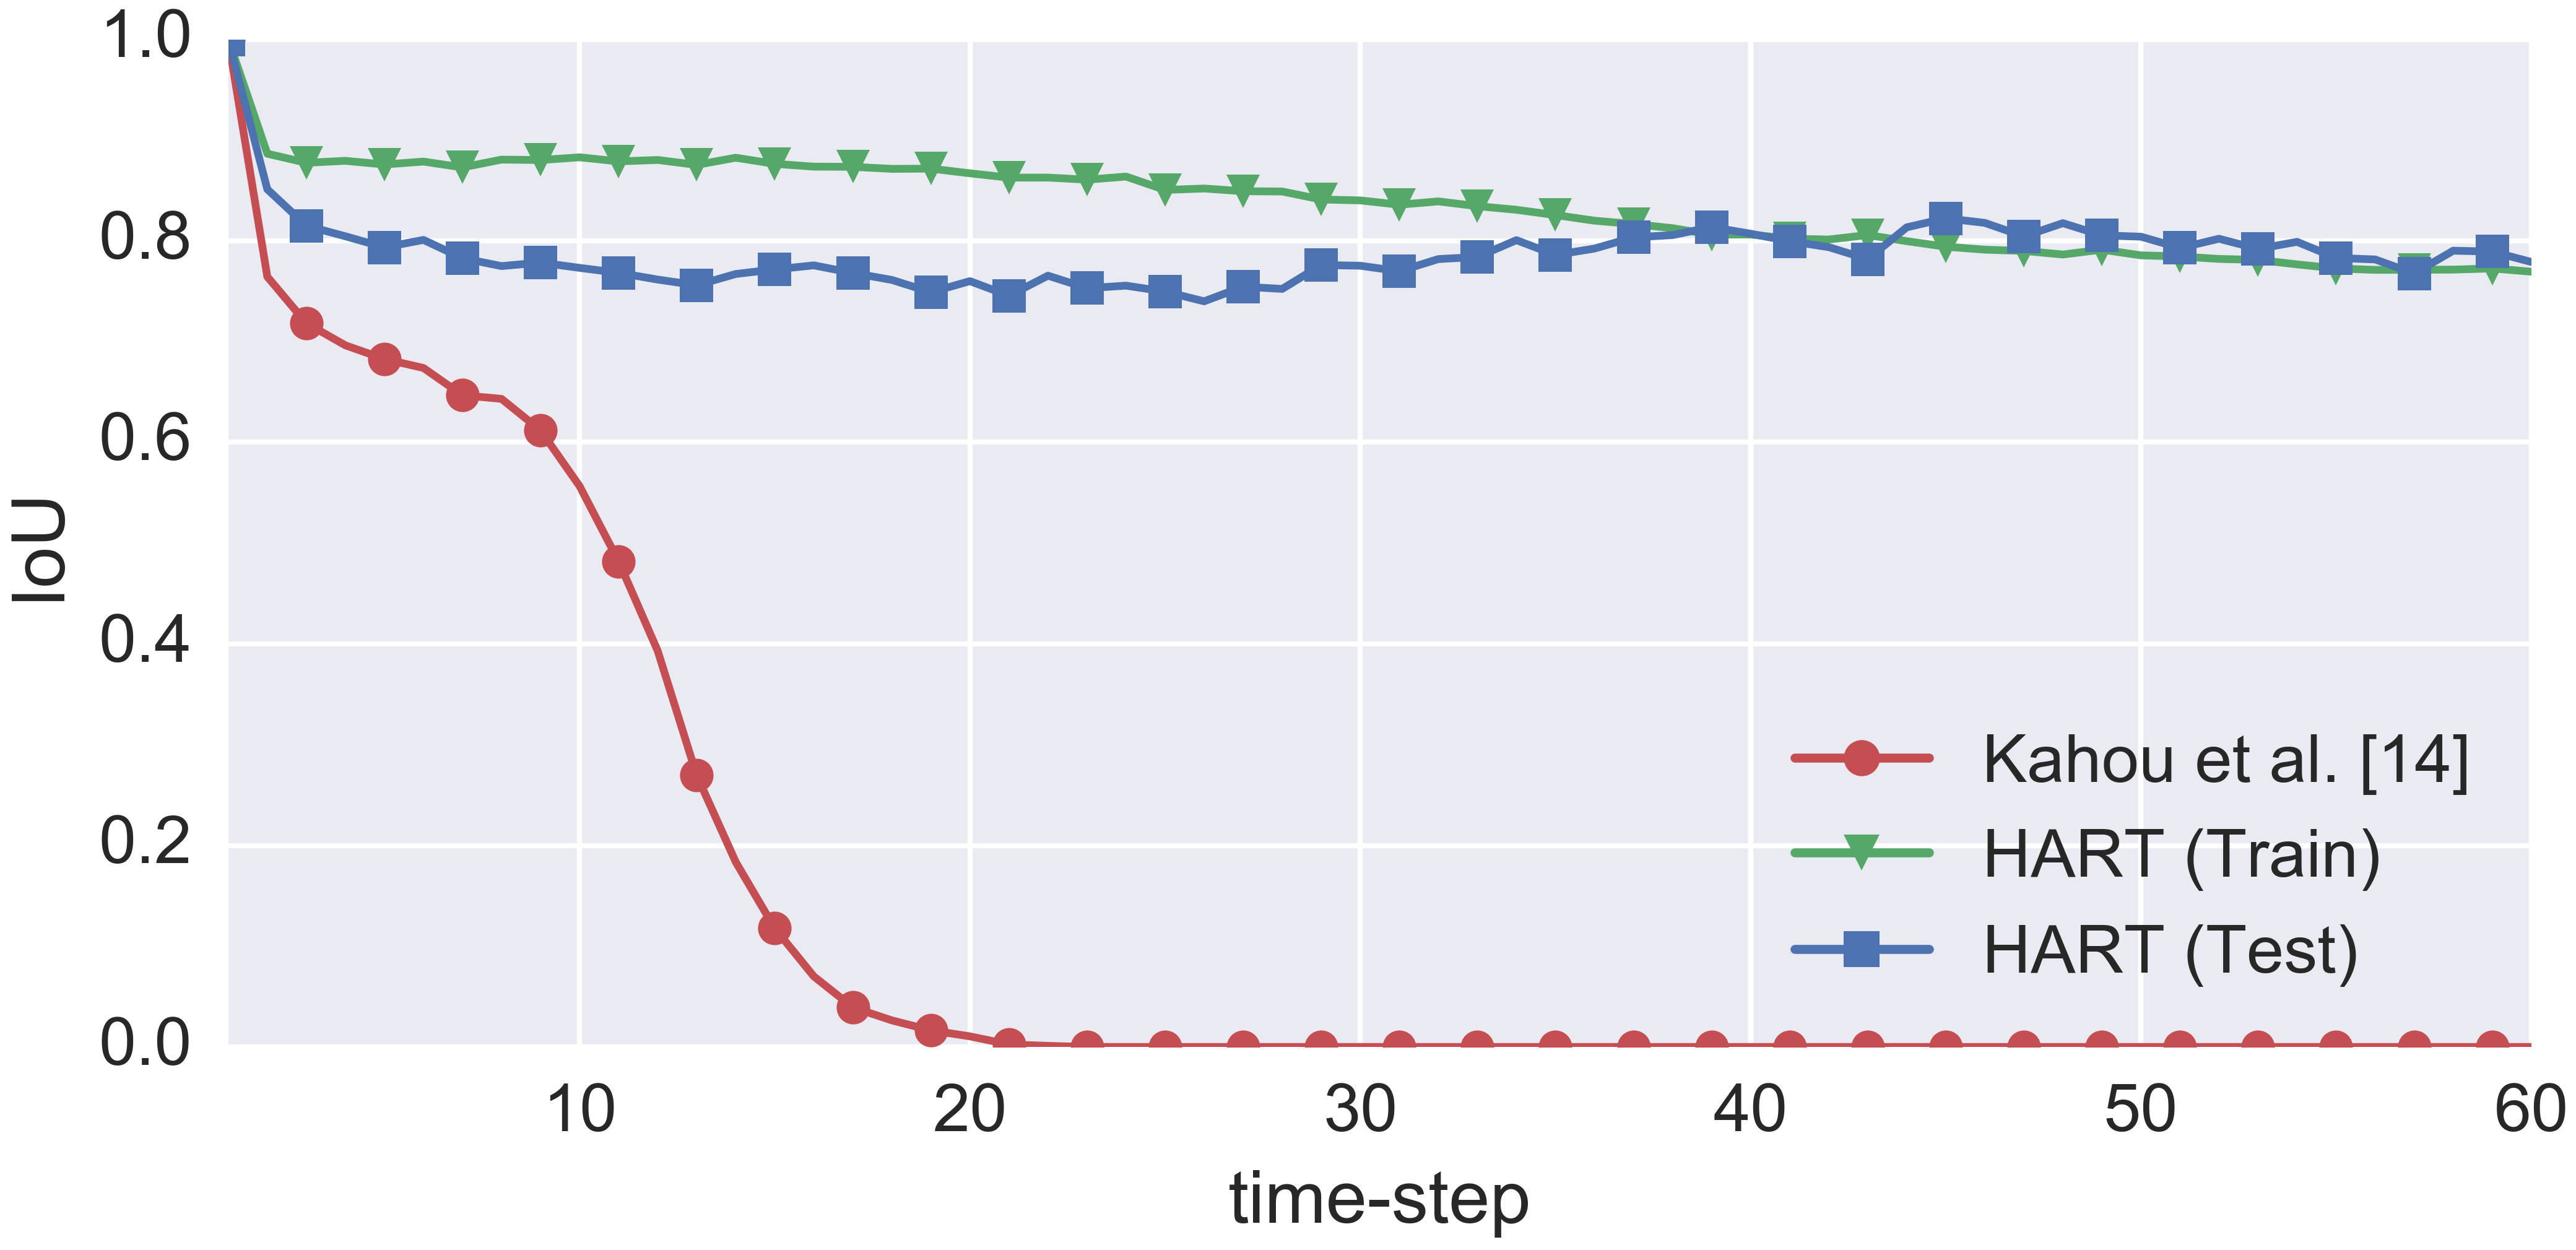
\includegraphics[width=\textwidth]{kitti_iou_fig}
        
        {\large
        \begin{minipage}[c]{0.5\linewidth}
            \centering
            \begin{tabular}{c|c|c|c}
                \multicolumn{4}{c}{Average IoU on KITTI over 60 time-steps}\\
                Kahou \emph{et. al.} [1] & Spatial Att & App Att & HART\\
                \midrule
                0.14 & 0.60 & 0.78 & \B{0.81}
            \end{tabular}
        \end{minipage}
        }\hfill
        \begin{minipage}[c]{0.4\linewidth}
            IoU curves on KITTI over 60 timesteps. HART~(train) presents evaluation on the train set.
        \end{minipage}
    \end{minipage}
    

    \vspace{1em}


%        \begin{tabular}{c|c}
%            \toprule
%            Method                      &   Avg. IoU\\
%            \midrule
%            \citet{Kahou2015ratm}       &   0.14      \\
%            Spatial Att                 &   0.60       \\  
%            % 			Spatial Att with Loss       &   0.70   \\
%            App Att                     &   0.78       \\
%            HART                        &   \B{0.81}   \\
%            \bottomrule
%        \end{tabular}
%        \vspace{1em}
%        Average IoU on KITTI over 60 time-steps.

%\mysection{Conclusion}

\begin{description}[labelsep=1em, leftmargin=!,labelwidth=\widthof{\bfseries Interpretable:}]
    \item[Bio-inspired:] Neural Recurrent tracking with\\ Attention Mechanisms.
    \item[Interpretable:] Important features selected by spatial attention and object segmentation mechanisms.
    \item[Scalable:] Auxiliary loss terms allow scaling to\\ complex real-world datasets.
    \item[Efficient:] $> 120$ fps on a laptop! 
    \item[Future Work:] Multi-object tracking.
\end{description}

\vspace{0\baselineskip}


\vspace{.5\baselineskip}

{\large References:}
{\small
\begin{description}
    \item[[1]] Samira Ebrahimi Kahoú, Vincent Michalski, and Roland Memisevic. RATM: Recurrent Attentive Tracking Model. CVPR Work., 2017.
    \item[[2]] Christian Schuldt, Ivan Laptev, and Barbara Caputo. Recognizing human actions: A local SVM approach. In ICPR. IEEE, 2004.
    \item[[3]] A. Geiger, P. Lenz, C. Stiller, and R. Urtasun. Vision meets robotics: The KITTI dataset. Int. J. Rob. Res.,
    32(11):1231–1237, sep 2013.
\end{description}
}

\end{multicols}

\end{poster}

\end{document}
